\documentclass[ENG,PhD]{cinvestav}

%%%%%%%%% PACKAGES
\usepackage{color}
\usepackage{latexsym, amssymb}
\usepackage{xcolor}
\usepackage{pstricks}
\usepackage{epsfig}
\usepackage{ucs}
\usepackage{lettrine}
\usepackage[utf8]{inputenc}
\usepackage{graphicx}
\usepackage{epstopdf}
\usepackage{url}
\usepackage{pseudocode}
\usepackage{ltablex}
\usepackage{rotating}
\usepackage{cite}

\RequirePackage{hyperref}
\RequirePackage{algorithm}
\usepackage{algorithmic}
\usepackage{fancybox}
\usepackage{pdflscape} 
\usepackage{multirow}
\usepackage{textcomp}
\usepackage{booktabs}
\usepackage{array}
\newcolumntype{L}[1]{>{\raggedright\let\newline\\\arraybackslash\hspace{0pt}}m{#1}}
\newcolumntype{C}[1]{>{\centering\let\newline\\\arraybackslash\hspace{0pt}}m{#1}}
\newcolumntype{R}[1]{>{\raggedleft\let\newline\\\arraybackslash\hspace{0pt}}m{#1}}
\usepackage{subcaption}

\usepackage[inline]{enumitem}
\newlist{listahorizontal}{enumerate*}{1}
\setlist[listahorizontal]{label=(\alph*)}

\newcommand{\V}[1]{\mathbf{#1}}

\graphicspath{ {../../../resources/images/vectors/}{../../../resources/images/bits/} }

\title{Smart Usage of Context Information for the Analysis, Design, and Generation of Power-Aware Policies for Mobile Sensing Apps}
\shorttitle{Smart Usage of Context Information for the Generation of Power-Aware Policies}
\author{Rafael Pérez Torres, César Torres Huitzil and Hiram Galeana Zapién}
\adscripcion{Cinvestav Tamaulipas. Parque Científico y Tecnológico TecnoTam -- Km. 5.5 Carretera Cd. Victoria-Soto La Marina. C.P. 87130 Cd. Victoria, Tamps. }
\city {Cd. Victoria, Tamaulipas, Mexico.}
%\date{December, 2010}
\techreportnumber{0}
\publishedmonth{December} %mes de la publicación
\publishedday{16th} %día de la publicación
\publishedyear{2015} %año de la publicación
\keywords{mobile sensing apps, energy consumption, context information, policy, smartphone}
\correspondingauthor{Rafael Pérez Torres $<$rperez@tamps.cinvestav.mx$>$, César Torres Huitzil $<$ctorres@tamps.cinvestav.mx$>$ and Hiram Galeana Zapién $<$hgaleana@tamps.cinvestav.mx$>$}
\grants{}
\dateofsubmission{December 16th, 2015}
\tobecited{Rafael Pérez Torres, César Torres Huitzil, Hiram Galeana Zapién. Smart Usage of Context Information for the Analysis, Design, and Generation of Power-Aware Policies for Mobile Sensing Apps. CINVESTAV Tamaulipas. 2014 Nov. 31 pp. (No Technical Report No. assigned)}
\placeanddateofpublication{Ciudad Victoria, Tamaulipas, MEXICO.}

\abstract{
This technical report describes the progress and advances developed for the thesis work titled \emph{Smart Usage of Context Information for the Analysis, Design, and Generation of Power-Aware Policies for Mobile Sensing Apps} during the first year of the doctoral program.

In summary, the different efforts during the first year have been focused on producing a solid state of the art revision, as well as on defining the core elements that will power up the methodology for solving the main problem.
}

\begin{document}
\makeintropages


% \subparagraph{Keywords.} mobile sensing apps, energy consumption, context information, policy, smartphone.

\section{Introduction}
\label{sec:introduction}
This technical report describes the progress and advances developed for the thesis work titled \emph{Smart Usage of Context Information for the Analysis, Design, and Generation of Power-Aware Policies for Mobile Sensing Apps} during the first year of the doctoral program.
In summary, the different efforts during the first year have been focused on producing a solid state of the art revision, as well as on defining the core elements that will power up the methodology for solving the main problem.

In order to ease the comprehension for the reader, this report has been structured as a self-contained document, including a summary of the scientific context of the research that describes the hypothesis, problem statement and objectives in Section~\ref{sub:research-context}.
Such summary also recalls the characteristics of smartphone-based sensing applications and the problematic aroused by the energy consumption when continuous access to sensors is needed.
Section~\ref{sec:state-of-art} is prepared as for describing the study performed on state-of-art techniques, covering a taxonomy of existing solutions, as well as a framework for their analysis.
Section~\ref{sec:methodology} is aimed at describing the refinements produced on our proposed solution, including the insights for achieving learning from user and a general overview of the mechanisms for achieving sensor usage adaptations.
Section~\ref{sec:preliminary-experimentation} presents the preliminary experimentation for ensuring the learning of mobility patterns in the mobile device.
Section~\ref{sec:future-work} describes the future work for achieving the planned solution.
Finally, Section~\ref{sec:conclusions} present the conclusions of this report.










% *************************************
% *************************************
% ****** 1. Research description ******
% *************************************
% *************************************
\section{Research description}
\label{sub:research-context}
\emph{This section is aimed at easing the comprehension of the document for the reader, giving an overall description of the context of the research, including problem statement, hypothesis, objectives, and contributions.}


The popularity of smartphones is a remarkable instance of the adoption of technology by society.
According to the Ericsson Mobility report~\cite{Ericsson2015} there were 3,400 million of smartphone subscriptions and 250 million of mobile PCs, tablets and mobile router subscriptions in the 2015.
The presence of smartphones is drastically changing our daily lives by providing an increasingly powerful set of tools as a result of significant advances in the field.
% It is expected to have 6,400 million and 350 million of subscriptions, respectively, by the end of the 2021.
The capabilities and platform complexity of smartphones are continuously improving, becoming truly system-on-chip (SoC) devices able to adapt their operation over three distinguishing dimensions, namely communication, sensing, and computation, as conceptually shown in Figure~\ref{fig:smartphone-dimensions}.
The advances on these dimensions have enabled the \emph{context-awareness}~\footnote{For the sake of clarity, we stick to the definition of \emph{context} proposed by Chen and Kotz~\cite{Chen2000}, as the set of environmental states and settings that either determines the application’s behavior or in which an application event occurs and is interesting to the user.} paradigm in mobile and pervasive computing, opening the path for a myriad of applications and services.
Particularly in the sensing dimension, modern smartphones include a set of low cost and powerful embedded sensors such as accelerometer, digital compass, gyroscope, GPS receiver, microphone, and camera, among others, providing them with rich capabilities for creating mobile sensing applications at different spatial and temporal scales~\cite{Lane2010,Campbell2012,Kjaergaard2012} and with different levels of accuracy and energy costs.
For this class of applications, the core requirements are the background and continuous sensors' data acquisition, as well as the associated on-device computations for extracting useful information for the user~\cite{Lane2010,Ra2012}.
As user interaction can be required for collecting data, two sensing paradigms can be implemented~\cite{Lane2010}.
The \emph{opportunistic paradigm} tries to determine the most appropriate moment for automatically collecting data from sensors without human participation at all.
On the other hand, the \emph{participatory paradigm} leverages user's abilities requiring his/her participation to describe data and choose the moment for collecting them.
Given its autonomy, the opportunistic paradigm represents the preferable choice for continuous mobile sensing.

\begin{figure}[t]
  \centering
  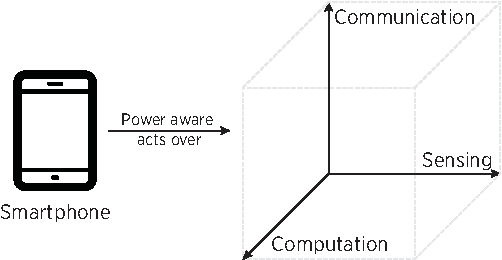
\includegraphics[scale=0.9]{smartphone-dimensions}
  \caption{The communication, computation, and sensing features offered by smartphones represent the main dimensions where the functionality of these devices relies on.}
  \label{fig:smartphone-dimensions}
\end{figure}


\subsection{Smartphone-based sensing characteristics}
Regardless of the sensing paradigm, the internal operation of mobile sensing applications commonly involves a set of stages that describe the closed loop shown in Figure~\ref{fig:stages-of-power-aware-mobile-sensing}, consisting in:
\begin{listahorizontal}
  \item \emph{Sensor reading} that involves selecting, configuring, and requesting data to sensors,
  \item An \emph{optional preprocessing} for discarding uninteresting data like outliers or reducing noise,
  \item \emph{Feature extraction} for obtaining features, i.e., more computationally efficient representations of data,
  \item \emph{Classification} of extracted features into classes of special interest, for example human activity aspects that might feed machine learning strategies, and
  \item \emph{Post-processing} for offering feedback to user, launching network communication, triggering another sensing-classification chain with the outcome of classification acting as feedback information for a more precise operation of sensors, or for performing further processing.
\end{listahorizontal}
At each stage, the level of context-awareness of the mobile platform is increased, requiring specific algorithmic solutions to perform the above described functions.
The design of such solutions is not straightforward, as there are a number of factors that impact the operation of each stage.
This is the case of the dynamics of user's context which depends on changes produced in the environment, the existing constraints in mobile platforms, and the privacy concerns of personal data manipulation that, as a whole, compromise the sensor readings, classification and post-processing of data.
Similarly, the implementation of these applications is hindered by priorities and additional requirements like the latency at which a context change is detected, the accuracy of the inferred context, and the implicit rational usage of energy resources.
\begin{figure*}[t]
    \centering
    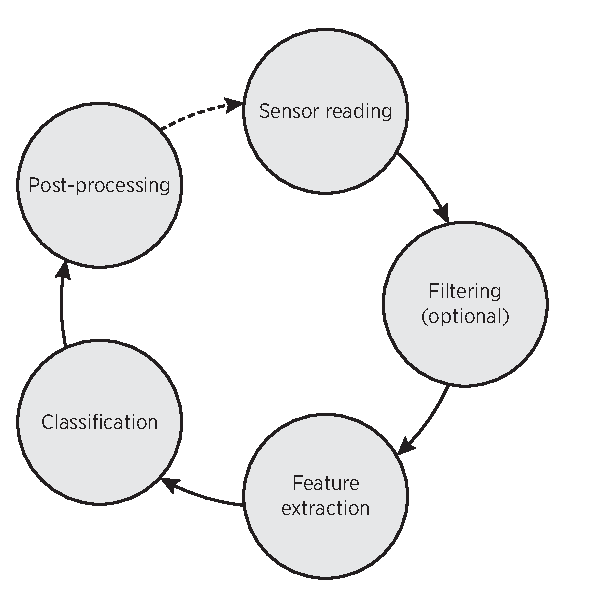
\includegraphics[width=\textwidth]{msa-stages}
    \caption{The different stages of mobile sensing applications produce output, shown in the lower gray rounded boxes, whose level of information is increasing at each stage. The post-processing stage might launch a new sensor reading chain as shown by the top dashed line.}
    \label{fig:stages-of-power-aware-mobile-sensing}
\end{figure*}

Despite the fact there is a common understanding of how to deploy the aforementioned stages in mobile sensing applications, the support for continuous sensing is still an open research problem due to the power demands of long-term sensing and the inherent resource-constrained characteristics of mobile devices.
Although modern smartphones feature increasing computing power, memory and longer battery life, the requirements of complex mobile sensing applications represent a great challenge for mobile platforms, especially to the battery consumption, whose typical capacity is on the order of thousands of mAh, growing only 5-10\% each year~\cite{Ma2012,Evarts2015}. 
This growing rate is not at the same pace than the advances in hardware and software components of mobile platforms, which in every new generation of mobile devices impose an ever growing energy demand.

At the same time, it is important to note that since their initial conception, mobile platforms described a layered architecture with a clear focus on managing the heavy interaction with user.
Because of this, the support for background running processes and for exploiting the power management capabilities existing at hardware level of sensors was discarded, leaving out the power-efficiency of the sensing dimension~\cite{Priyantha2011}.
As a consequence, efficient implementations of power-aware mechanisms that do not jeopardize the accuracy requirements of mobile sensing applications still remain an open challenge, which is augmented by the computational and power constraints of mobile devices, as well as the long-term and near real-time requirements of these applications.


\subsection{Hypothesis} 
\label{sub:hypothesis}
As described in previous section, long-time operation of mobile sensing applications remains as an open challenge, due to the inherent trade-off between the energy consumed when accessing to sensors and the accuracy of the activity being tracked.
In simpler terms, the more accuracy obtained when accessing sensors with high frequency, the higher energy consumption.
Nonetheless, this research work considers that the dynamics of context information inferred from sensors data is of remarkable value for adapting sensory operations and producing power savings.
Thus, the hypothesis pursued in this thesis states that \emph{intelligent policies produced through context information built from sensors data can be employed to reduce the energy consumption in a mobile device when performing continuous sensor readings}.

In a deeper description, a smart policy is a special rule that defines how sensors should be accessed in order to reduce the energy consumption and achieve mobile app requirements.
This research work aims to employ data coming from GPS and inertial sensors in order to obtain context information in terms of mobility patterns, useful to reduce the energy consumption generated by LBS's~\footnote{LBS, Location Based Service.}.


\subsection{Problem statement} 
\label{sub:problem_statement}
In order to prove the aforementioned hypothesis, this research work identifies the existence of two interrelated problems, which are described as follows.
The first one is depicted as a \emph{pattern identification problem} and is focused on detecting changes in the mobility pattern of user from sensors data.
Such pattern represents the context information that is helpful to add \emph{smartness} to the policies that adapt sensory operations.

Formally:
Given a set $V = \left\{v_{1}, v_{2}, \dotsc, v_{n}\right\}$ of data values read from sensor $S$ in the time interval $T  \in [t_{1}, t_{2}]$, identify the current mobility pattern $p_{S}$ that represents the activity of user.

\begin{equation}
  PatternIdentifier( V ) \longrightarrow{} p_{S} \in Patterns
\end{equation}

Where $Patterns$ is a set of patterns that represent an interesting state in user mobility, specifically the set $\left\{no\_movement, walking, running, vehicle\_transportation\right\}$.

On the other hand, the \emph{policy generation problem} is related to the selection and configuration of proper sensors for keeping the user location tracking, while at the same time reducing energy consumption.
For this process, it is also important to consider the level of the smartphone's battery and the accuracy requested by the mobile application.

Formally:
Given the set of detected mobility patterns $\mathcal{P} = \{ p_{S_1}, p_{S_2}, \ldots, p_{S_n} \}$ in data from sensors $\mathcal{S} = \{ S_1,S_2,\ldots, S_n \}$, accuracy required $a$, and physical constraints status $c$ of a mobile device, find a policy that select the proper set of sensors $\mathcal{S}_{new}$ and its associated configuration $\mathcal{S}_{new_{conf}}$  while meeting application requirements.

\begin{equation}
  PolicyGeneration( \mathcal{P}, a, c ) \longrightarrow{} \mathcal{S}_{new}, \mathcal{S}_{new_{conf}}
\end{equation}

The $\mathcal{S}_{new_{conf}}$ configuration is referred as the \emph{adaptive duty cycle} of associated sensor.


\subsection{Objectives} 
\label{sub:objectives}

\subsubsection*{Main objective}
\label{ssub:main_objective}
To reduce energy consumption in the mobile sensing apps, which perform continuous sensor readings, through self-adapting power-aware policies generated from context information obtained from sensors data.

\subsubsection*{Particular objectives} 
\label{ssub:particular_objectives}
\begin{itemize}
  \item To identify mobility patterns from context information obtained from an inertial sensor (accelerometer) and location providers (GPS, WPS).
  \item To generate policies for a self-adapting sensors' usage from identified mobility patterns, accuracy and energy requirements of mobile application, and status of mobile device's constraints. 
  \item To ease the development of mobile sensing applications that require user location tracking, i.e., LBS, isolating the complexity of sensors' access and the associated efficient energy management.
\end{itemize}


\subsection{Contributions} 
\label{sub:contributions}

\begin{itemize}
  \item A mechanism for detecting mobility patterns from the data read by sensors of mobile devices (specifically GPS and accelerometer).
  \item A mechanism for generating policies for accessing sensors.
  Such mechanism employs application requirements (energy and precision hints), level of mobile device constraints, and user's context information (using the pattern detected by previous mechanism).
  The produced policies will allow to perform a smarter usage of smartphone's sensing infrastructure in continuous sensor readings, reducing the energy consumption.
  \item A middleware that implements the previously described mechanisms, easing the development of mobile sensing applications.
\end{itemize}










% *************************************
% *************************************
% ****** 2. State of art related ******
% *************************************
% *************************************
\section{State-of-art works analysis}
\label{sec:state-of-art}
\emph{The content of this section describes the results of the analysis of state-of-art related works. A taxonomy of these solutions is presented, and the pure hardware and hardware-software approaches are briefly described. Finally, the pure software approach is presented at detail, highlighting its advantages over other approaches, and including a framework for decomposing and studying solutions under this category.}


\begin{figure*}[t]
  \centering
  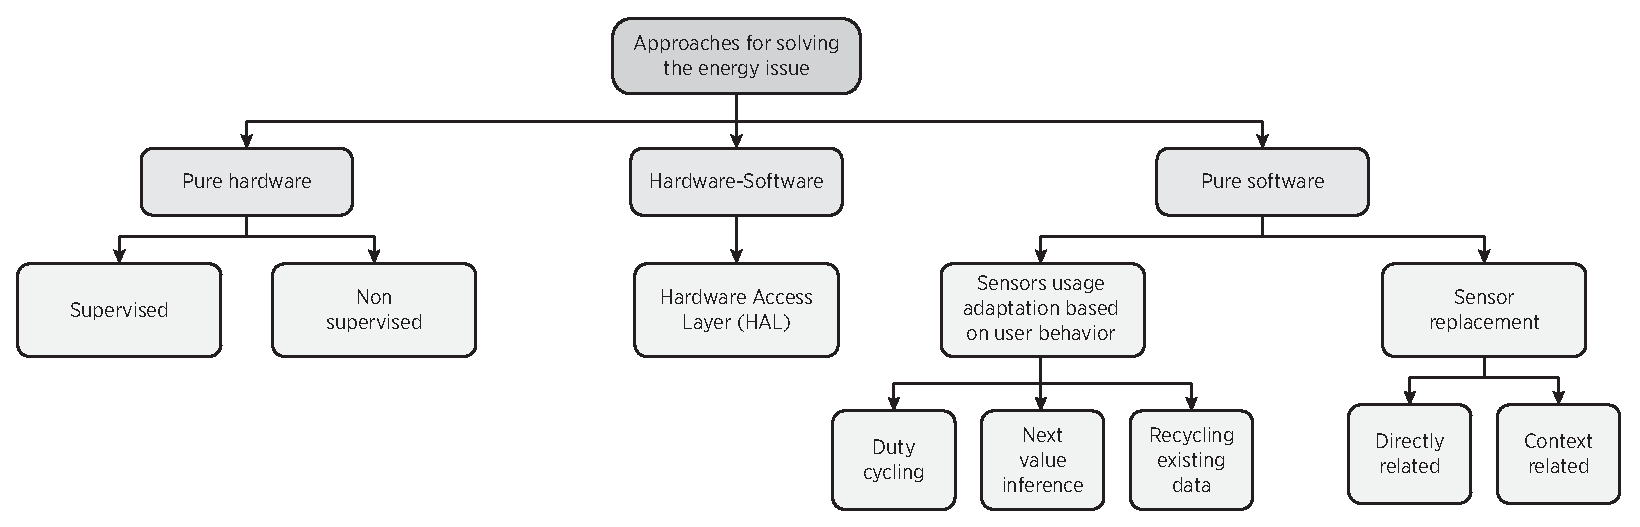
\includegraphics[width=\textwidth]{approaches-taxonomy}
  \caption{The taxonomy of solutions for power-aware smartphone sensing is divided into three categories: pure hardware, hardware-software and pure software.}
  \label{fig:taxonomy-approaches}
\end{figure*}

\emph{Power-aware sensing} refers to the set of techniques aimed at continuously monitoring sensor data over long periods of time under the computing, storage, and power constraints of typical mobile devices.
Roughly speaking, the power-aware sensing is mostly enclosed into the sensor reading stage of mobile sensing applications (highlighted in red in the Figure~\ref{fig:stages-of-power-aware-mobile-sensing}), abstracting the complexity of sensors management, and delivering collected data while considering the power constraints of these devices. 
It is important to remark that such goal is frequently achieved by executing the rest of the stages internally, in order to identify context information useful for feedback purposes and a smarter usage of sensors.

% A revision of relevant works in literature reveals three complementary approaches at different level of abstraction of the smartphone device: pure hardware, hardware-software, and pure software approaches.
Figure~\ref{fig:taxonomy-approaches} presents a taxonomy of solutions found in literature for power-aware smartphone-based sensing, with the pure hardware, hardware-software and pure software approaches as the main classes.
%It has been identified that the support for these policies at system level of a mobile platform facilitates the analysis, control, and cross-layer coordination and information sharing for reducing the power consumption, which is the reason why power-aware sensing mechanisms should be supported throughout all layers of the mobile platform~\cite{Ranganathan2010}.
The distribution of each of these approaches across the layers of a mobile platform is depicted in Figure~\ref{fig:distribution-approaches}, highlighting the increasing support in the higher layers for reacting accordingly to the dynamics of context information through more complex and robust machine learning mechanisms.
% The distinctive characteristics of the different approaches are as follows:
\begin{figure}[t]
  \centering
  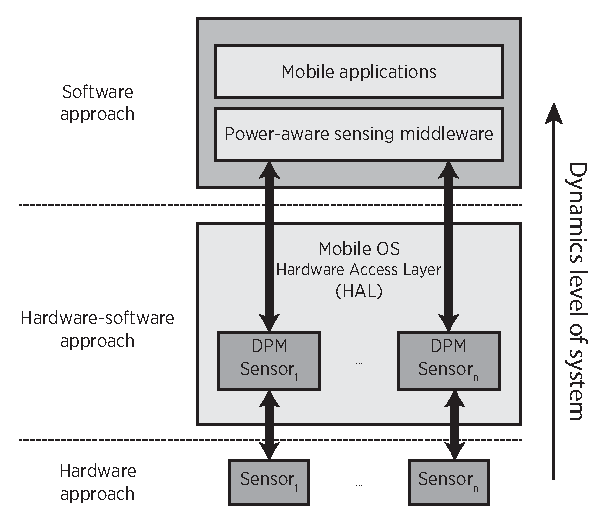
\includegraphics[width=0.5\columnwidth]{approaches-distribution}
  \caption{The approaches distributed across the mobile platform stack are more adaptive to system's dynamics on the higher layers.}
  \label{fig:distribution-approaches}
\end{figure}
% \begin{itemize}
%   \item The \textbf{pure hardware approach} is the lowest level at which power-aware optimizations could be performed.
%   It involves the selection of power-aware sensors and embedded components to deliver physical data to upper layers of mobile platform, as well as the definition of the different power modes of the hardware components through techniques like Dynamic Voltage and Frequency Scaling (DVFS)~\cite{Priyantha2011,Choi2010}.
%   Such power modes define a static behavior of hardware components, which can be adapted through hardware control points exported to upper layers, as in~\cite{Priyantha2011,Choudhury2008,Apple2015}.
%   \item The \textbf{hardware-software approach} abstracts fine grain details and isolates the usage of hardware components for mobile applications and upper platform layers.
%   This isolation is performed by applying system-wide policies that coordinate the operation and interaction of the whole set of sensors according to dynamic changes in their workload and global status of the mobile platform (like battery level).
%   The hardware-software approach is aware of the hardware components of the mobile platform, and is able to define DPM mechanisms for turning sensors on and off, and adapt their configuration parameters, as proposed in~\cite{Ra2012,Zhuang2010}.
%   \item The \textbf{pure software approach} is aimed at modeling, identifying and even predicting details about context information and its dynamic changes from sensor data, in order to define smart mechanisms for power-aware adaptation of the hardware components usage, like the implementations by~\cite{Chon2014,Yurur2014,MaY2009}.
%   Because of the fully context-awareness that this approach achieves, it is able to obtain high levels of flexibility for adaptive management of sensors, and put the context information detected from sensors data at service of the whole mobile platform.
% \end{itemize}
It is important to recall that although the presented taxonomy allows to classify the power-aware smartphone-based sensing techniques, the relevance of this problem makes that in practice many of the solutions combine different strategies pursuing an integral and better power management.
% This is a suggestion of the complexity of the problem itself and an evidence of the evolution and adoption of these complementary techniques.
% Furthermore, ideas proved to be working efficiently in software soon or later are implemented directly in hardware to boost efficiency even further. 
% http://bit.ly/1M2sLVr
%\newgeometry{left=1.7cm}
\begin{table*}
    \centering
    \scriptsize{}
    
    %\begin{tabular}{C{0.07\linewidth}C{0.21\linewidth}C{0.28\linewidth}C{0.2\linewidth}C{0.1\linewidth}}
    \begin{tabular}{C{0.09\linewidth}C{0.17\linewidth}C{0.25\linewidth}C{0.18\linewidth}C{0.17\linewidth}}
    \toprule
    \textbf{Year} & \textbf{Name} & \textbf{Mobile platform} & \textbf{Description} & \textbf{Approach} \\
    \midrule
    \cite{Choudhury2008} 2008 & \emph{The Mobile Sensing Platform} & Intel iMote with custom hardware & User motion & Pure hardware \\
    \cmidrule(l){1-5}
    \cite{Priyantha2011} 2011 & \emph{LittleRock} & Not specified & User motion & Pure hardware \\
    \cmidrule(l){1-5}
    \cite{Apple2015} 2013 & \emph{Apple iPhone 5s} & Apple iPhone 5s and newer & User motion & Pure hardware \\
    \cmidrule(l){1-5}
    \cite{Zhuang2010} 2010 & Not given & Android G1 (Android 1.5) & User location & Hardware-Software \\
    \cmidrule(l){1-5}
    \cite{Ra2012} 2012 & Not given & Samsung SGH-i917 (Windows Phone 7.5) & Generic sensors access & Hardware-Software \\
    \cmidrule(l){1-5}
    \cite{Constandache2009} 2009 & \emph{EnLoc} & Nokia N95 (Symbian 60) & User location & Pure software \\
    \cmidrule(l){1-5}
    \cite{Abdesslem2009} 2009 & \emph{SenseLess} & Nokia N95 (Symbian 60) & User location & Pure software \\
    \cmidrule(l){1-5}
    \cite{Wang2009} 2009 & \emph{EEMSS} & Nokia N95 (Symbian 60) & User location, user activity & Pure software \\
    \cmidrule(l){1-5}
    \cite{Kjaergaard2009} 2009 & \emph{EnTracked} & Nokia N95 (Symbian 60) & User location & Pure software \\
    \cmidrule(l){1-5}
    \cite{MaY2009} 2009 & \emph{iLoc} & Simulation & User location & Pure software \\
    \cmidrule(l){1-5}
    \cite{Paek2010} 2010 & \emph{RAPS} & Nokia N95 (Symbian 60) & User location & Pure software \\
    \cmidrule(l){1-5}
    \cite{Kim2010} 2010 & \emph{SensLoc} & Simulation & User location & Pure software \\
    \cmidrule(l){1-5}
    \cite{Perez2010} 2010 & \emph{G-Sense} & Simulation & User location, user activity & Pure software \\
    \cmidrule(l){1-5}
    \cite{Lin2010} 2010 & \emph{A-Loc} & Simulation and Android G1 & User location & Pure software \\
    \cmidrule(l){1-5}
    \cite{Lu2010} 2010 & \emph{Jigsaw} & Nokia N95, Apple iPhone & User location, user activity & Pure software \\
    \cmidrule(l){1-5}
    \cite{Chon2011} 2011 & \emph{SmartDC} & HTC Desire (Android 2.1) & User location & Pure software \\
    \cmidrule(l){1-5}
    \cite{Paek2011} 2011 & \emph{CAPS} & Nexus One (Android 1.5-2.2) & User location & Pure software \\
    \cmidrule(l){1-5}
    \cite{Srinivasan2012} 2012 & Not given & Simulation & User activity & Pure software \\
    \cmidrule(l){1-5}
    \cite{Perez-Torres2012} 2012 & Not given & Samsung Galaxy S (Android 2.3) &  User location & Pure software \\
    \cmidrule(l){1-5}
    \cite{Zhang2013} 2013 & \emph{SensTrack} & Google Nexus S (Android 4.1.4) & User location & Pure software \\
    \cmidrule(l){1-5}
    \cite{Mazilu2013} 2013 & \emph{Not given} & Custom Samsung Galaxy Nexus, and Samsung Galaxy S4 (Android) & User location & Pure software \\
    \cmidrule(l){1-5}
    \cite{Chon2014} 2014 & \emph{FreeTrack} & Smartphone not specified (Android 2.2) & User location & Pure software \\
    \cmidrule(l){1-5}
    \cite{Man2014} 2014 & Not given & Samsung Galaxy III (Android 4.1.4) & User location & Pure software \\
    \cmidrule(l){1-5}
    \cite{Yurur2014} 2014 & Not given & Blackberry Storm II & User activity & Pure software \\
    \cmidrule(l){1-5}
    \cite{Donohoo2014} 2014 & Not given & HTC MyTouch 3G, Google Nexus One, and others (Android) & User location, user activity & Pure software \\
    \cmidrule(l){1-5}
    \cite{AlvarezDeLaConcepcion2014,Morillo2015} 2014 & Not given & Google Nexus One & User activity & Pure software \\
    \cmidrule(l){1-5}
    \cite{Khalifa2015} 2015 & Not given & Simulation (of energy harvesting device) & User activity & Pure software \\
    \bottomrule
    \end{tabular}
    \protect\caption{A set of produced works aimed at solving the power consumption issue in smartphone-based mobile sensing. Most of the solutions follow a pure software approach, given its flexibility and adaptive features.\label{tab:related-work}}
    
\end{table*}
%\restoregeometry

Table~\ref{tab:related-work} summarizes a set of works found in literature aimed at solving the power consumption issue in mobile sensing applications in the context of the presented taxonomy.
As it can be noted, the most common strategy followed in the literature is the pure software approach, due to its flexibility and fine-tuning capabilities.
Also, because of the heterogeneity of target features, main purpose, mechanisms for measuring power savings, and mobile platforms where the mechanisms proposed in each work were implemented, it is not straightforward to perform a fair comparison among them~\cite{Vallina-Rodriguez2013,Neely2008}.
The different approaches of this taxonomy are described in the following sections.
% For example, the solutions may target a different set of sensors or the techniques for analyzing context information produce outputs with different semantic meaning.
% Also there is no a clear consensus for measuring the energy benefits of proposed solutions; in this regard two main strategies have been followed.
% The first and most common strategy is to perform a comparison in terms of mW between energy consumed by a solution and the mobile platform or a similar approach. 
% However, even inside this strategy the implementations are not homogeneous and the proposed solutions employ different methods for measuring energy consumption in mobile devices, namely highly-invasive, moderately-invasive, and non-invasive techniques, as described in~\cite{Abreu2012}.
% The second strategy performs the comparison in terms of battery life (e.g., time to drain) because, according to~\cite{Kim2014}, several physical characteristics of batteries impact on their discharging cycle.
% The most notorious aspect is that the actual available energy is reduced when the battery discharges, a behavior that is ignored in the energy consumption models included in most of the reviewed solutions.



\subsection{Pure hardware approach}
The fundamental idea behind the pure hardware approach is the selection of power-aware hardware elements for providing physical data to upper layers of the mobile platform, as well as the definition of mechanisms to adapt the hardware input parameters, like DVFS.
These mechanisms allow the creation of control points for manipulating hardware usage, which are known as power modes~\cite{Ranganathan2010,Lorch1998,Benini2000}.
The mobile platform keeps the list of power modes fixed and instruct sensors to work isolated from others.
In this way, the hardware components obey a static behavior defined only through power modes, whose control points are exported to upper layers of the mobile platform.

The set of works under this approach typically involve the design of specific hardware to exploit the aforementioned features.
This design implies the isolation of the components associated with the measurement of physical signals inside a new unit with a dedicated low power processor (LPP).
Since the mobile OS isolates the access to these hardware components, mobile applications remain agnostic about the new hardware unit and can consume its power-aware sensing services without modifying their inner logic.
The basic behavior of this unit requires sensors to report their readings to the embedded LPP, which is capable of executing light preprocessing operations like noise filtering.
While the hardware unit performs the reading and filtering stages, the rest of the smartphone hardware platform is able to reach its sleep mode, producing power savings.
Table~\ref{tab:works-hardware-approach} shows some of the most representative works under the pure hardware approach.
Depending on the ability to process data and discover contextual information autonomously, the pure hardware approach can be implemented in two different ways, namely the \emph{ad-hoc data acquisition} and the \emph{co-processing} variants, as shown in Figure~\ref{fig:taxonomy-approaches}.

\begin{table}[t]
    \centering
    \scriptsize{}
    \begin{tabular}{C{0.25\columnwidth}C{0.2\columnwidth}C{0.4\columnwidth}}
    \toprule
    \textbf{Name} & \textbf{Variant} & \textbf{Sensors involved} \\
    \midrule
    LittleRock \cite{Priyantha2011} & Ad-hoc data acquisition &  Accelerometer, compass, gyroscope \\
    
    Apple iPhone 5s \cite{Apple2015} & Coprocessing & Accelerometer, compass, gyroscope \\

    The Mobile Sensing Platform \cite{Choudhury2008} & Coprocessing & Accelerometer, barometer, compass, humidity, light, microphone, temperature \\
    \bottomrule
    \end{tabular}
    \protect\caption{Representative works under the pure hardware approach. More context-aware features are being deployed directly into hardware components of mobile platforms.\label{tab:works-hardware-approach}}
\end{table}


The \emph{\textbf{ad-hoc data acquisition}} variant is restricted to serve the different mobile application requests for raw sensor data, discarding the analysis and extraction of higher level information.
% For instance, \emph{LittleRock}, proposed by Priyantha \emph{et al.}, in~\cite{Priyantha2011}, defines a specific unit with embedded sensors powered directly from battery, allowing the main circuitry of the smartphone to reach the sleep mode while performing sensor readings.
% Once a special event defined by a mobile application is detected in data coming from sensors, \emph{LittleRock} is able to wake up the phone for further processing.
% \emph{LittleRock} is faster than the phone itself to collect a single sample of data from sensors, due to the complexity of the software stack that smartphone's main processor has to handle.

Besides the raw data delivery, the \emph{\textbf{co-processing}} variant adds support to hardware layers for light data processing and detection of higher level information, producing context-awareness at hardware level with low power consumption.
In this sense, the sensing facilities of the hardware platform are transformed into smart sensors~\cite{Gervais-Ducouret2011}.
The embedded LPP of the sensing unit must be powerful enough to perform such analysis.
Smartphone manufacturers have begun to integrate into the device's hardware full suites of sensing capabilities.
For instance, Apple has implemented a platform re-design of the \emph{iPhone} smartphone, which starting at \emph{5s} version features an isolated sensing unit able to process sensor data and deliver fitness information like the amount of steps and distance covered by user, as well as the type of activity performed, namely, stationary, walking, running, automotive, cycling, and unknown~\cite{Apple2015}.
% In addition to this hardware platform update, the Software Development Kit (SDK) of iPhone exposes this functionality through a software Application Programming Interface (API) denominated the \emph{CoreMotion Framework} that enables mobile applications to request and consume the fitness information.
% A similar co-processing mechanism is implemented by Choudhury \emph{et al.}, in the \emph{Mobile Sensing Platform} (\emph{MSP})~\cite{Choudhury2008} which employs ad-hoc components for building a custom mobile sensing platform with a LPP able to perform light classification tasks for identifying user activity.

Regardless of the variant, a common aspect taken into account in the design of pure hardware approach solutions is the power consumption-usage generality trade-off that emerges when hardware designers are unable to foresee the needs of any future mobile application and implement power-aware mechanisms to support them directly in the circuits.
Because of this limitation, the effort of designers is focused on implementing general features that can be employed by many mobile sensing applications, instead of very specific features meaningful only for a few of them.

\subsection{Hardware-software approach}

The hardware-software approach is aimed at defining system-wide policies for deciding when to turn sensors on and off, or when to switch to a different power mode of a given hardware component.
In this level, the hardware-software approach is aware of the existence of different sensors and coordinates the basic operations and interactions between them, being able to abstract fine grained parameters into a coarser grained set, isolating the hardware usage for mobile applications and elements in upper platform layers.
Unlike the pure hardware approach, the hardware-software approach offers a basic understanding of global activities being performed by the mobile device, and also an implicit observance of dynamic changes in the workload of hardware components for deciding when to adapt hardware operation.
Because of the coupled interaction with hardware components of the platform, hardware-software approach solutions are produced as HAL's of the mobile OS or low level middlewares that build an interface that abstracts the access to sensors and isolates their complex management mechanisms.
Table~\ref{tab:works-hardware-software-approach} presents a few instances of works that follow this approach.
\begin{table}
    \centering
    \scriptsize{}
    \begin{tabular}{C{0.2\columnwidth}C{0.4\columnwidth}C{0.25\columnwidth}}
    \toprule
    \textbf{Reference} & \textbf{Produced HAL} & \textbf{Sensors involved} \\
    \midrule
    \cite{Ra2012} & API for selecting processor for execution of arbitrary tasks & Accelerometer, microphone \\
    
    \cite{Zhuang2010} & Automatic substitution, suppression, piggybacking, and adaptation of location providers & GPS, wireless interface \\
    
    \bottomrule
    \end{tabular}
    \protect\caption{Representative works under the hardware-software approach. The produced hardware interfaces improve the overall efficiency of the mobile platform.\label{tab:works-hardware-software-approach}}
\end{table}


% An example of the hardware-software approach is the inclusion of software mechanisms that leverage a dedicated LPP for accessing and manipulating sensors data.
% The software mechanisms allow to build the basic global status of the mobile platform, which is employed for manipulating the hardware through the control points exposed by sensors.
% Since the LPP can be powered independently of smartphone's main circuitry, it can execute tasks while the rest of the mobile platform can reach the idle state, producing potential energy savings.
% The work presented by Ra \emph{et al.}~\cite{Ra2012}, leverages the presence of such LPP's in the latest smartphones, putting their computing facilities at service of mobile applications through a layered API. 
% Any processor with a small wake-up transition delay could be suitable to be used as a LPP, and will achieve the highest power savings when executing the most frequent and lightest computations, like sensor sampling requests and simple filtering.

% Zhuang \emph{et al.}, presented in~\cite{Zhuang2010} a hardware-software approach middleware for LBS's execution based on the next four key design principles: 
% \begin{listahorizontal}
%   \item \emph{Sensor Substitution}: It allows on-the-fly substitution of current location provider with another with lower energy consumption and an accuracy level enough for the mobile application requirements,
%   \item \emph{Sensor Suppression}: Avoids usage of any location provider by leveraging data from energy cheaper sensors, like the accelerometer, for revealing when user is static,
%   \item \emph{Sensor Piggybacking}: It allows to serve location updates to simultaneous LBS's, and
%   \item \emph{Sensor Adaptation}: It reacts to low battery levels to adapt system-wide sensing parameters like time and distance.
% \end{listahorizontal}
% For identifying places where it is possible to substitute a location provider, it relies on a novel concept referred to as the \emph{M-Area} which defines a geographical zone along with information about the available location providers on it.
% The size of these areas involves a trade-off between the sensor substitution events and the storage space needed to save their information.

\subsection{Pure software approach}
Thanks to the context information obtained from sensor data, the pure software approach can bring activity awareness to the mobile platform and make informed decisions for fully dynamic power-aware sensors management as illustrated in Figure~\ref{fig:distribution-approaches}, where the pure software approach is at the top of the hierarchy.
Typically, pure software approach solutions are powered up by a set of classifiers fed with sensors data that individually identify basic aspects or produce abstractions about user activity.
Such user activity aspects are the fundamental elements for defining sensor management policies.
% In this way, the pure software approach is able to make the mobile platform aware about user activity and even adapting accordingly to changes on its profile.
In power-aware computing terms, the pure software approach can be understood as \emph{spending power to save power}~\cite{Ranganathan2010}.
In this sense, there is an unavoidable amount of energy that is spent while performing computational tasks for preprocessing, classifying and discovering context information from sensor data.
However, the acquisition of such context information is valuable as for improving the awareness of the smartphone about high level user activities~\cite{Yurur2014c}.
% Solutions following this approach can only observe the details of the hardware platform exposed by the hardware access or lower layers of the mobile OS.
% A practical interpretation can be expressed as follows: these lower layers know how to turn circuits on and off, but are unable to define when; whereas the higher software layers are flexible and can dynamically adapt to changes in user context, knowing when adapt the sensors operation, but delegating how to do it to the lower layers.
Pure software approach solutions are commonly implemented through a layered middleware with classification and machine learning modules embedded on it, as depicted in Figure~\ref{fig:middleware-software-approach}.
This middleware is placed between running mobile applications and the sensing and communication layers of the mobile platform, abstracting its sensing and communication facilities~\cite{Yurur2014}.
The different variants found in the pure software approach are described in the next section.

\begin{figure}
  \centering
  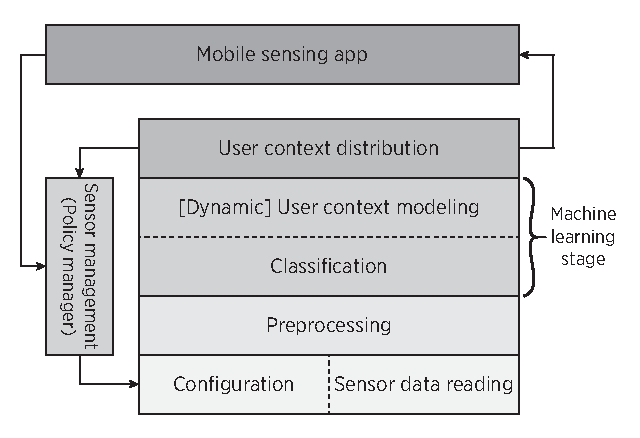
\includegraphics[width=0.5\columnwidth]{generic-middleware-architecture}
  \caption{A generic structure of a middleware following a pure software approach defines explicit modules for selecting and configuring sensor access, and classification and machine learning stages.}
  \label{fig:middleware-software-approach}
\end{figure}




\subsubsection{Categories of the pure software approach}
\label{sub:software-categories}
Depending on the type of decision made for modifying sensory operations, two variants of the software approach can be identified, namely the \emph{Sensor usage adaptation} and \emph{Sensor replacement}.

% \checkmark
% http://bit.ly/1CCoRAP
\begin{sidewaystable}
% \begin{table*}
    \centering
    \scriptsize{}
    \begin{tabular}{C{0.11\textwidth}C{0.2\textwidth}C{0.17\textwidth}C{0.15\textwidth}C{0.09\textwidth}C{0.05\textwidth}C{0.05\textwidth}C{0.05\textwidth}}
    % \begin{tabular}{C{0.15\textwidth}C{0.22\textwidth}C{0.25\textwidth}C{0.27\textwidth}}
    \toprule
    \textbf{Name} & \textbf{Variants} & \textbf{Machine learning technique} & \textbf{Sensors involved} & \textbf{Complexity} & \textbf{OL} & \textbf{OO} & \textbf{US} \\
    \midrule

    
    % Category Basic context policy (short time window)
    \emph{G-Sense}      \cite{Perez2010} & Sensor adaptation (DC) & SDR & GPS & low \\

    \cmidrule(l){1-8}
    Not given           \cite{Perez-Torres2012} & Sensor adaptation (DC) & SDR & GPS & low \\

    \cmidrule(l){1-8}
    \emph{SenseLess}    \cite{Abdesslem2009} & Sensor adaptation (DC), Sensor replacement (CR, DR) & SDR & WPS, GPS, ACC & low \\
    
    \cmidrule(l){1-8}
    \emph{SensTrack}    \cite{Zhang2013} & Sensor adaptation (DC), Sensor replacement (CR, DR) & SDR & ACC, orientation sensor, GPS, WPS & low \\
    % \emph{SensTrack}    \cite{Zhang2013} & Sensor adaptation (DC), Sensor replacement (CR,DR) & SDR, Gaussian Regression Model (GRM) & ACC, orientation sensor, GPS, WPS & low \\
    
    \cmidrule(l){1-8}
    Not given           \cite{Man2014} & Sensor adaptation (DC, VI), Sensor replacement (CR) & SDR & ACC, magnetic field sensor, GPS & low \\
    % Not given           \cite{Man2014} & Sensor adaptation (DC), Sensor replacement (CR) & SDR (Trigonometrical approach) & ACC, magnetic field sensor, GPS & low \\

    \cmidrule(l){1-8}
    \emph{EnLoc}        \cite{Constandache2009} & Sensor adaptation (DC, VI), Sensor replacement (DR) & SDR, Mobility Tree & WPS, GPS, cellular ID & medium & & \checkmark \\
    
    \cmidrule(l){1-8}
    \emph{EnTracked}    \cite{Kjaergaard2009} & Sensor adaptation (DC), Sensor replacement (CR) & SDR & ACC, GPS & medium & & \checkmark \\
    \bottomrule


    % Category Medium context-aware policy
    % Not given           \cite{AlvarezDeLaConcepcion2014,Morillo2015} & --- & Ameva algorithm, majority vote system & ACC & low \\
    Not given           \cite{AlvarezDeLaConcepcion2014,Morillo2015} & --- & Ameva algorithm & ACC & medium \\
    
    \cmidrule(l){1-8}
    Not given           \cite{Mazilu2013} & Sensor replacement (CR) & DT & Temperature, humidity, pressure & medium \\
    % Not given           \cite{Mazilu2013} & Sensor replacement (CR) & DT (C4.5) & Temperature, humidity, pressure & medium \\

    \cmidrule(l){1-8}
    Not given           \cite{Srinivasan2012} & Sensor adaptation (DC) & DT & ACC & medium \\
    
    \cmidrule(l){1-8}
    Not given           \cite{Khalifa2015} & Sensor replacement (CR) & KNN & Model of ACC-based harvesting device & medium \\
    % Not given           \cite{Khalifa2015} & Sensor replacement (CR) & KNN & Model of ACC-based harvesting device & low \\
    \bottomrule


    % Category Long time window
    \emph{SensLoc}         \cite{Kim2010} & Sensor adaptation (DC, RD), Sensor replacement (CR) & SDR & Wi-Fi fingerprinting, GPS, ACC & medium & \checkmark & \\
    % \emph{SensLoc}         \cite{Kim2010} & Sensor adaptation (DC), Sensor replacement (CR,DR) & SDR (Tanimoto coefficient and ACC variance) & Wi-Fi fingerprinting, GPS, ACC & medium & \checkmark & & \checkmark \\
    
    \cmidrule(l){1-8}
    \emph{CAPS}         \cite{Paek2011} & Sensor adaptation (DC, RD), Sensor replacement (CR) & SDR & GPS, cellular ID & medium & \checkmark \\
    % SDR (Smith-Waterman algorithm) CR because location is processed alternatively with this algorithm

    \cmidrule(l){1-8}
    \emph{RAPS}         \cite{Paek2010} & Sensor adaptation (DC, RD), Sensor replacement (CR, DR) & SDR & WPS, GPS, ACC, Bluetooth, cellular ID & medium & \checkmark \\
    
    % In-between Category Optimization + long time window
    \cmidrule(l){1-8}
    \emph{A-Loc}        \cite{Lin2010} & Sensor adaptation (DC, RD), Sensor replacement (CR, DR) & HMM, Bayesian estimation framework & GPS, WPS, Bluetooth, cellular ID & medium & \checkmark & \checkmark  \\
    
    \cmidrule(l){1-8}
    \emph{SmartDC}      \cite{Chon2011} & Sensor adaptation (DC, RD), Sensor replacement (CR, DR) & HMM and LZ predictor & GPS, WPS, Wi-Fi and cellular ID fingerprinting & medium & \checkmark & \checkmark \\

    
    \bottomrule


    % Category Full context-aware policy
    \emph{Jigsaw}       \cite{Lu2010} & Sensor adaptation (DC), Sensor replacement (CR) & Microphone: NB with Gaussian Mixture Model (GMM). ACC: DT. GPS: MDP. & ACC, Microphone, GPS & high & & \checkmark & \checkmark \\
    
    \cmidrule(l){1-8}
    Not given           \cite{Donohoo2014} & Sensor adaptation (DC) & Several. KNN and NN selected as best. & ACC, GPS, WPS, cellular ID, light, device data, mobile app requirements & high & & & \checkmark \\

    \cmidrule(l){1-8}
    \emph{EEMSS}        \cite{Wang2009} & Sensor adaptation (DC), Sensor replacement (CR, DR) & GPS and ACC: SDR. \newline Microphone: SSCH algorithm. & ACC, microphone, GPS & high & & & \checkmark \\

    \cmidrule(l){1-8}
    \emph{iLoc}         \cite{MaY2009} & Sensor adaptation (RD), Sensor replacement (CR) & HMM & Wi-Fi \& GSM fingerprinting & high & \checkmark & & \checkmark  \\
    
    \cmidrule(l){1-8}
    Not given           \cite{Yurur2014} & Sensor adaptation (DC, RD) & HMM & ACC & high & \checkmark & & \checkmark \\
    
    \cmidrule(l){1-8}
    \emph{FreeTrack}    \cite{Chon2014} & Sensor adaptation (DC, RD), Sensor replacement (CR, DR) & HMM & GPS, Wi-Fi, cellular ID, battery status & high & \checkmark & & \checkmark \\
    
    \bottomrule
    \end{tabular}
    \protect\caption{Important works proposed following the pure software approach. Many of these works combine different software strategies for boosting their energy performance. (OL: Online Learning from user data, OO: Optimization Oriented solution, US: User State context insight, ACC: Accelerometer).\label{tab:works-software-approach}}
% \end{table*}
\end{sidewaystable}


\paragraph{Sensor usage adaptation}
It is based on the analysis of historical data in a time window for detecting patterns or events in the user behavior.
Once a pattern is detected it can be employed in the three following ways for adapting sensors usage and reduce power consumption:
\begin{itemize}
  \item \emph{\textbf{Duty cycling (DC)}}:  The frequency for accessing sensors is reduced, introducing sleep periods in hardware, and hence achieving power savings.
  However, this also produces the accuracy - power consumption trade-off, since the continuous data acquisition is interrupted and mobile applications would work with such data gaps.
  \item \emph{\textbf{Next value inference (VI)}}: Obtains an inference of the next value to be delivered by sensors, avoiding an actual access to them, and hence reducing power consumption; however, this introduces uncertainty to the system which may be not acceptable for certain applications.
  Typically, the inference is produced by probabilistic measures focused on low level dependencies observed in short-time windows of raw sensor data.
  \item \emph{\textbf{Recycling existing data (RD)}}: Identifies common circumstances or events in high level context information that happened previously, reusing data from such events.
  In practice, this is feasible since people describe a consistent behavior, which can be identified by looking at patterns in their activities in long time windows~\cite{Chon2011,Paek2011}.
  Since actual access to sensors is avoided, it may also introduce uncertainty to the system if the probability of accurately identifying the event is low.
\end{itemize}

\paragraph{Sensor replacement}
It permits a replacement of the sensor currently employed for collecting data with another one that consumes less power and has immediate data availability.
Replacing a sensor may involve the definition of a mapping function between the data type of the selected sensor and the replaced one.
Such mapping function is needed when the output of sensors is not compatible; for instance, accelerometer data can used for inferring distance, but only after proper processing (integrating for speed and position).
Depending on whether such mapping is needed, two specializations can be found:
\begin{itemize}
  \item \emph{\textbf{Directly related replacement (DR):}} The sensor is replaced with a lower energy hungry one that delivers the same data type and guarantees the application's accuracy requirements, without the need of a mapping procedure.
  \item \emph{\textbf{Context related replacement (CR):}} The type of the data returned by the selected sensor is not as expected by the application, implying a mandatory procedure for translating it to the requested data type.
\end{itemize}

A noteworthy aspect about pure software approach solutions is that typically once their power efficiency is proved in tests and real life implementations, they might be implemented in the hardware or lower layers of the mobile OS.
For instance, modern inertial sensor devices incorporate an internal buffer that allows data queuing until it is full or the phone is woken up; also, recent GPS receivers are able to implement \emph{geo-fencing} features directly in hardware~\cite{Torroja2013}, allowing to wake up the smartphone when it enters in the geo-fenced area.
Both functionalities were initially available in the Android platform via software but now are supported at hardware level~\cite{Android2013,Developers2014}.
Also, lower layers of newer versions of Android allow the \emph{piggy-backing} of close in time GPS requests, reusing the same GPS fix\footnote{A GPS fix is a location point obtained through the GPS infrastructure.} for concurrent mobile applications~\cite{Zhuang2010}. 
This transference of platform functionalities from software to hardware is always subject to the aforementioned trade-off between the generality of features and power saving benefits: a very generic mechanism can be suitable for any mobile application but will not obtain the largest power savings; on the other hand, the best power savings are obtained by the most specific and tuned solutions that may result useless for the rest of mobile application scenarios.

Table~\ref{tab:works-software-approach} shows a set of works following the pure software approach.
For the sake of brevity, the next section focuses on describing a set of important features found in these works and a framework for studying them, rather than presenting a comprehensive review of each work.

\subsubsection{Relevant characteristic of the software approach}
The openness and flexibility of the software stack of mobile devices allows to implement a wide variety of strategies and mechanisms that can dynamically adapt to changes detected in context information.
In addition to such diversity of strategies, there is also heterogeneity in the scenarios (like LBS, HAR\footnote{HAR, from Human Activity Recognition.}, crowd sensing) and objectives pursued by the different pure software solutions, which hinders their review and makes it hard to produce a definitive framework for their analysis.
As an example of this heterogeneity, the reader can consider works that duty cycle sensors usage.
In some proposed solutions, the context information employed in the policies for adapting duty cycle is simple, even raw data with simple heuristics; while on the other hand, some solutions build and process a more complex model of context information before performing a decision with more robust classifiers.
In this way, we identify that the granularity (or the level) of context information represents the pivotal feature on which the analysis and description of works can be performed.

The granularity of context information can be mostly characterized by the combination of the next elements: 
\begin{listahorizontal}
  \item the data type of the input directed to classifiers,
  \item the classifier itself, and
  \item the length of the time window employed to sense data.
\end{listahorizontal}
Recall that although solutions can follow unconstrained combinations over these elements for inferring context information, at the end the mechanisms for adapting sensors operation will incur into one or more variants of the pure software approach, described in Section~\ref{sub:software-categories}.
Also, it is worth noting that among the different features described by solutions, the following attributes are helpful to analyze and understand core features of their design and operation.
First, solutions can incorporate mechanisms for online learning (OL) from context information, enabling predictive features thanks to observance over long-time windows of sensory data.
Also, works can follow and optimization orientation (OO) approach in order to formalize, for instance, a sensor usage adaptation (replacement) mechanism and guarantee a given target in terms of minimum energy consumed and/or the error in activity tracking.
Finally, the solutions might employ an enriched version of the context information, known as user state (US) for allowing the device to become fully activity-aware and ease its adaptation over the sensing dimension.
% Siento que una debilidad que aun tenemos es la "definición" de US, lo cual sin duda tenemos que especificar en el planteamiento de la solución. Aquí sin embargo está débil. Y recordemos también que lo que intentamos aquí es que el US está relacionado a movilidad, dada la crítica de uno de los revisores
With the previous elements in mind, a framework aimed at studying the different modules of software solutions can be developed.
Figure~\ref{fig:framework-pure-software-solutions} presents an overview of the components of such framework.
In the \emph{Machine Learning for Context-Awareness} module, the solutions implement classifiers or mechanisms that allow them to gain understanding of context information.
These classifiers can act over short time windows of sensors data, analyzing what the user is doing at the current time interval.
Also, the length of such time window can be longer, involving a learning of context information that help to produce more robust inferences about user activity.
At the end, regardless of the length of the time window and the complexity of the information learned, this module directs the context information to the \emph{Policy generator} module.

The \emph{Policy generator} module is focused on processing the incoming context information (and other parameters like accuracy and energy requirements) for producing a better selection and configuration of sensors that derive in energy savings.
Again, the internal mechanism can be simple or complex, following probabilistic and even classic optimization paradigms.
The outcome of this module is materialized as one or more of the pure software variants shown in Figure~\ref{fig:distribution-approaches}.


Finally, the \emph{Hardware adaptation} module receives the configuration specified by the \emph{Policy generator} and applies it to the sensing infrastructure of the smartphone in order to produce power savings.

In this way, the different software solutions produced in literature can be decomposed and observe at their differences employing this framework.
As a final comment, recall that the flexibility of the software platform allow solutions to implement any combination of techniques in each module according to their particular objectives and scenarios.

\begin{figure}[t]
  \centering
  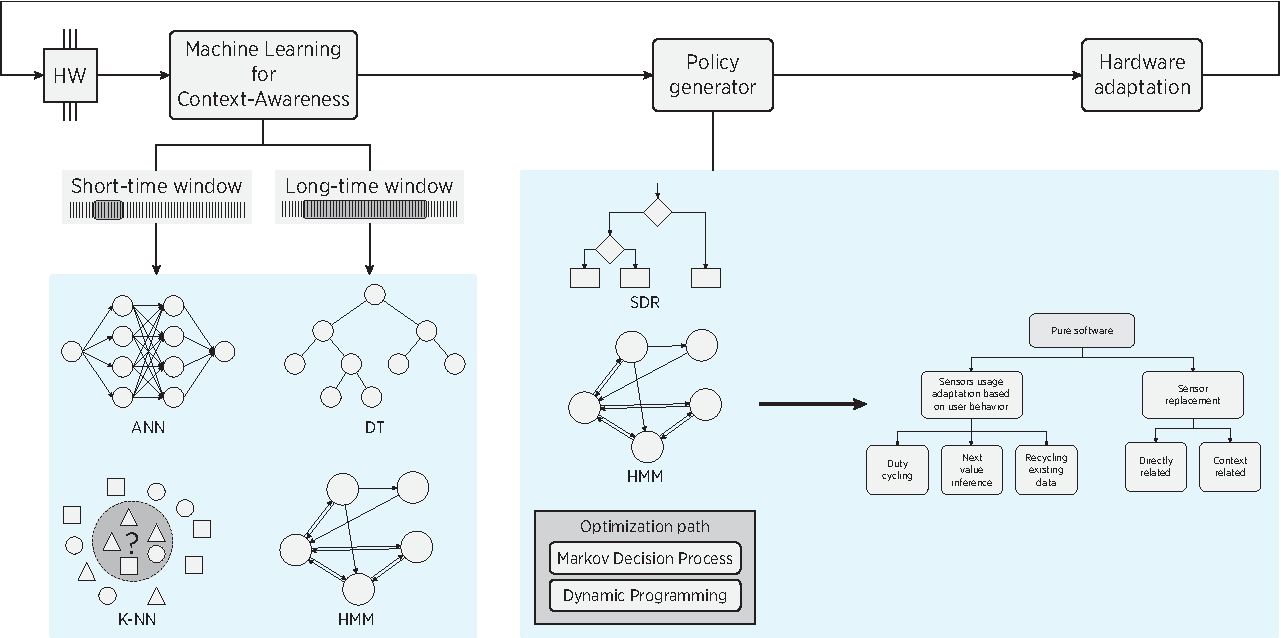
\includegraphics[width=\textwidth]{dual-taxonomy-clean}
  \caption{Framework for analyzing and studying the building components of pure software solutions.}
  \label{fig:framework-pure-software-solutions}
\end{figure}










% *************************************
% *************************************
% ***** 3. Advances in methodology ****
% *************************************
% *************************************
\section{Refinement of methodology}
\label{sec:methodology}
\emph{This section presents the refinements developed in the methodology aimed at solving the problem of interest of this thesis work.}

After reviewing the different solutions proposed in literature, it is possible to define a clear perspective for solving the main problem of this research, including the underlying model of the mobility information learned from user, as well as the strategies for adapting the sensing operation.
In order to clarify the scope of this research, it is important to state that a pure software approach will be followed, given its flexibility for detecting and adapting to changes detected from context information.

\subsection{Overview of the proposed solution}

The first relevant aspect to consider is that the overall problem can be decomposed into two main challenges.
In one hand, it is needed to learn and identify the different points of interest in user mobility.
On the other hand, it is also critical to perform the tracking of user while moving between these points.
In this way, the continuous location tracking leverages on the points of interest as \emph{anchor points} representing the origin and destination of each user trajectory.
Every time the user enters into a place of interest, the GPS-based tracking can be stopped and employ additional sensors and strategies for ensuring that user remains at such place while reducing power consumption.
When user leaves the place, the location tracking can be restarted but also observing at the learned information for predicting the next possible place and employ this information for improving access the access to location providers.

\begin{figure}[t]
  \centering
  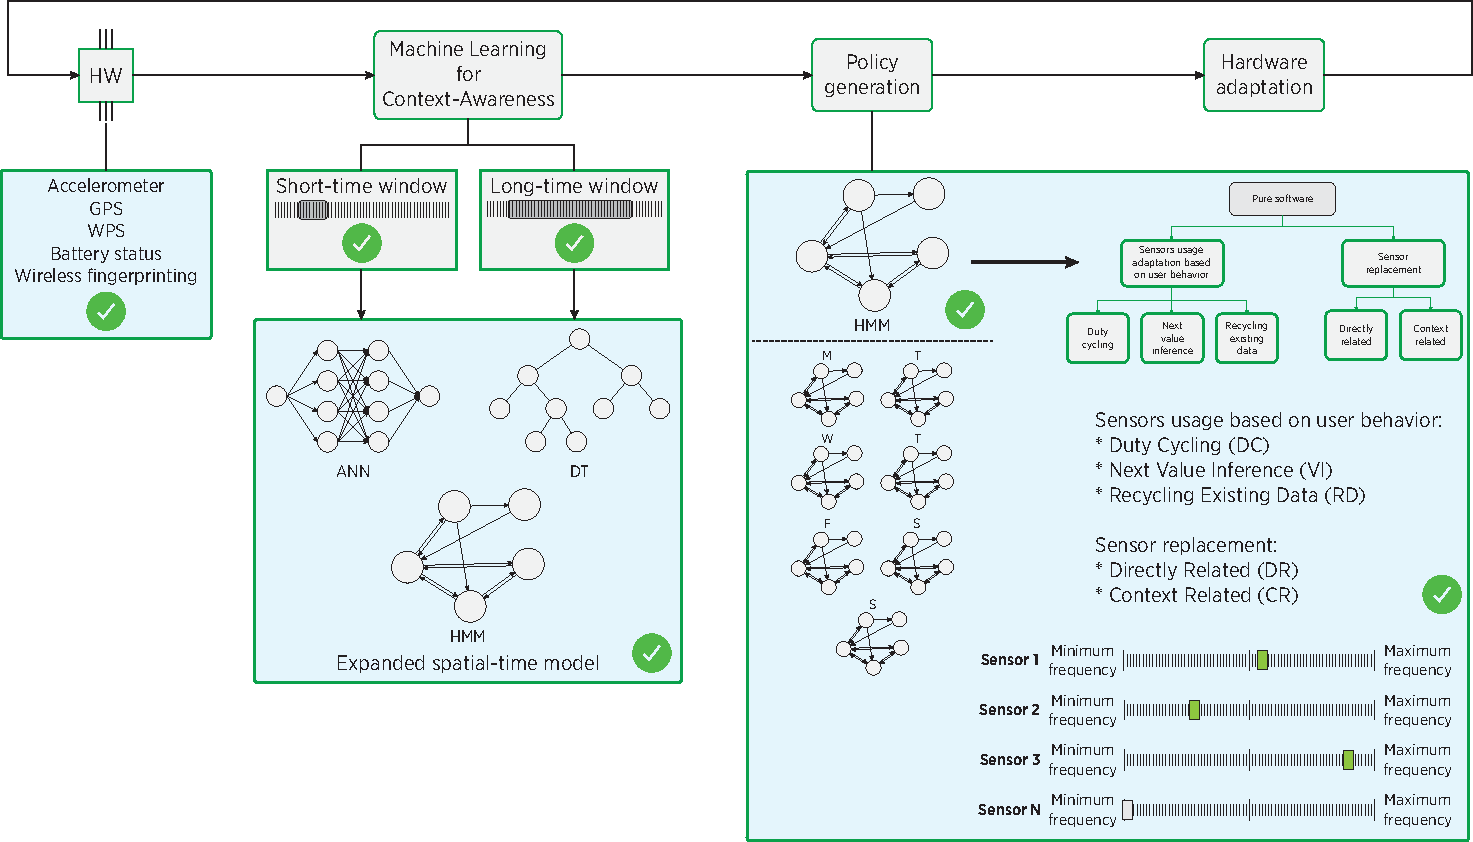
\includegraphics[width=\textwidth]{dual-taxonomy-ours}
  \caption{Decomposition of our solution.}
  \label{fig:decomposition-our-solution}
\end{figure}

Figure~\ref{fig:decomposition-our-solution} shows the different characteristics of the proposed solution employing the framework described in previous section.
As can be seen, the sources of context information to be employed are the accelerometer, GPS and WPS location providers.
However, also the battery status and wireless fingerprinting will be used for aiding the arrival to points of interest as follows.
Wireless fingerprinting can represent the signature of a place through the strength of the signal of available access points; the smartphone continuously keep a list of such network devices that when compared with existing signatures can detect whether the smartphone is at a previous known location.
In the case of battery status, it is noteworthy that users tend to charge his/her smartphone in particular places like home and work, which allows to avoid unnecessary GPS readings.

In the \emph{Machine Learning for Context-Awareness} module, Artificial Neural Networks (ANN) and Decision Trees (DT) will be employed to analyze short time windows of sensors data for detecting user activity.
Hidden Markov Models (HMM) will be used for understanding the transitions between frequent stay points in user mobility.
The detection of stay points will be performed employing adaptations of classic GPS trajectory analysis algorithms, like the proposed in~\cite{Montoliu2010}.
It is important to mention, than the user mobility is not to be modeled through classic HMM, but instead employing a custom expanded spatial-time model, as depicted in Figure~\ref{fig:expanded-spatial-time model}.
This spatial-time model not only keeps context information about places in pure location aspects (i.e., latitude and longitude) but also in terms of time context, like arrival, departure, and average stay time.
Also, the spatial-time model enriches the information available for the transitions between places, including aspects like the described motion (i.e., way of transportation) for a fine grain tuning of sensing operations.
Also, note in Figure~\ref{fig:decomposition-our-solution} the existence of particular models for each day of the week, given the differences in the mobility patterns described by people in weekdays and weekends.

\begin{figure}[t]
  \centering
  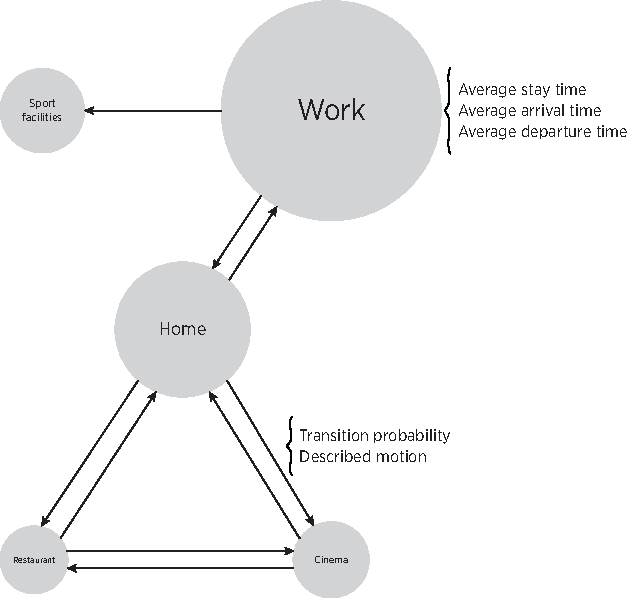
\includegraphics[scale=0.85]{mobility-graph}
  \caption{Expanded spatial-time model as the building block of learned information in the proposed solution.}
  \label{fig:expanded-spatial-time model}
\end{figure}

Finally, in the \emph{Policy generation} module, the probability of transition between learned places will play a critical role for determining a more adequate set of sensors (and associated configuration) that derives in energy savings and the fulfillment of the accuracy requirements of the mobile app.
Each of the variants existing in the pure software approach will be implemented, recalling the options for replacing the GPS through wireless fingerprinting and the status of the battery.
In practice, the proposed solution looks for defining upper and lower thresholds in the sampling frequency of sensors, keeping their operation inside such intervals and making the proper adaptations with the aid of context-aware policies.


\subsection{Architecture of the proposed solution}
\begin{figure}[t]
  \centering
  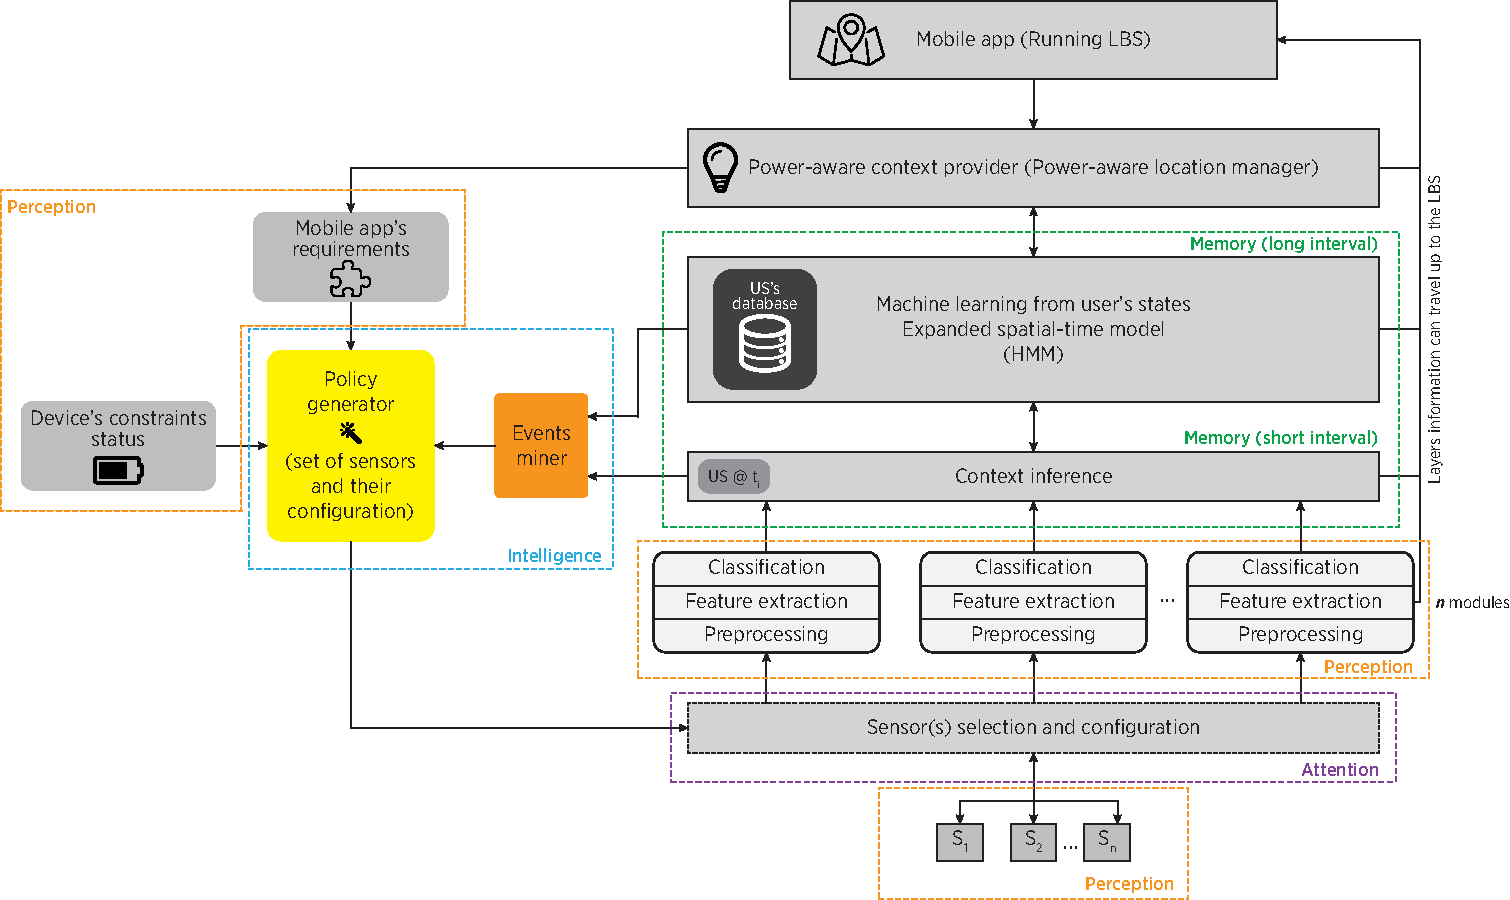
\includegraphics[width=\textwidth]{solution-general-overview}
  \caption{Architecture of the proposed solution.}
  \label{fig:solution-architecture}
\end{figure}

The different elements depicted in previous section are integrated in the architecture shown in Figure~\ref{fig:solution-architecture}.
Note that there are several classification modules, one per sensor, which will obtain hints or aspects about the status of user.
The outcome of these modules is directed to the \emph{Context inference} block, where it is integrated for inferring the current situation of the user (User state, US).
Such current state is delivered to the \emph{Policy generator} block and to the \emph{Machine Learning} block.

The \emph{Machine Learning} block uses the information received from the \emph{Context inference} block for building and enhancing the spatial-time model of user mobility, learning his-her mobility patterns.
Such task is done, by using HMM augmented with time dimension information as described in previous section.
This block also delivers the learned information to the \emph{Policy generator} module.

The \emph{Policy generator} is in charge of defining the next set of sensors and their associated configuration for keeping the tracking of user within the accuracy interval specified by the running mobile app.
This block employs current information obtained from sensors (current US) and the historical information maintained in the system (expanded spatial-time model), in order to improve the management of sensors.
% The battery level is also of special interest for this block in order to ensure the reduction in the energy consumption.
Sensing operation is adapted also depending in the battery level, producing a lower sampling frequency when the battery is low.

All this architecture is providing location updates to mobile apps in a power-aware manner.
Running mobile apps only have to specify the accuracy requirements to the architecture by interacting with the \emph{Power-aware location manager} interface, which will inform of this requirement to the \emph{Policy generator} block.
At the end, the running mobile app is agnostic about all the processes running in the background for collecting and analyzing context and location data, receiving the location updates transparently.
Also, the mobile app can receive the outcome produced in each layer of the architecture for specific tasks and further processing.


\section{Preliminary experimentation}
\label{sec:preliminary-experimentation}
\emph{This section presents a description of the preliminary experimentation performed for validating the possibility of learning mobility patterns solely in the mobile device.}


An important advance developed during the current period is an experimentation focused on ensuring that the learning of the spatial time model is factible in the mobile device.
Particularly, an on-device detection of points of interest (also referred as stay points) was pursued through the design of an event-oriented middleware, whose architecture is shown in Figure~\ref{fig:on-device-stay-point-detection-architecture}.
This middleware has been implemented for the Android platform, which allows the access to smartphone's sensors in an asynchronous manner.

\begin{figure}[t]
  \centering
  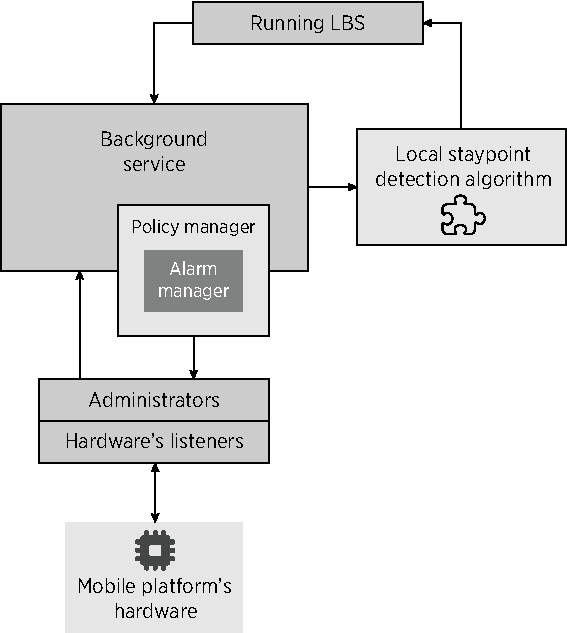
\includegraphics[scale=0.75]{architecture-for-gps-policies}
  \caption{Architecture for on-device detection of points of interest.}
  \label{fig:on-device-stay-point-detection-architecture}
\end{figure}


As such, the middleware permits mobile applications to register for stay points notifications by employing a callback mechanism, and autonomously manages the access to GPS receiver, stopping the collection of data and turning it of when needed.
The overall operation of our architecture can be summarized as follows.
First, the running LBS communicates to a background running service for requesting the user location tracking and stay points detection.
Then, the background service instructs a policy manager for starting the collection of data. 
After receiving each GPS fix, it is delivered to the running LBS as well as to the stay point detection module for further processing.

More specifically, the components of the architecture perform the following activities.
First, the policy manager module is in charge of two main tasks.
In one hand, it dispatches the initial request from the background service for collecting GPS data and also manages the scheduling of next GPS readings through sensor access policies.
On the other hand, it registers the scheduled readings as alarms (through the \verb|ALARM_MANAGER| service) in the Android software stack in order to obtain an actual adaptive sensing.
Such alarm manager strategy is needed since the design of the Android platform implements aggressive power-saving restrictions in order to extend the battery life.
For our particular task it becomes relevant that an Android-enabled mobile device might reach its sleep power mode and would disable further scheduled readings.
This is where the alarms become helpful, since they represent a mechanism for re-activating the mobile device from sleep mode and trigger the execution of needed tasks.
However, mobile device still can reach sleep mode while collecting and processing GPS data.
The Android platform provides a special token denominated partial \verb|WakeLock| that, when acquired, forces the CPU and low-level hardware components to be activated (except for the screen, which is kept turned off), allowing the middleware to
\begin{listahorizontal}
  \item trigger a GPS update,
  \item process the data for scheduling a new GPS update with the aid of a reading policy, and
  \item release the \verb|WakeLock| for allowing the device to reach its sleep mode again.
\end{listahorizontal}

The hardware's listeners and administrator layers are developed for controlling the registration-unregistration with hardware facilities of the smartphone, remaining agnostic about the rest of activities performed by the mobile platform.

%With the aid of this middleware, the running LBS only needs to instruct the background service for starting GPS readings, and then receive such updates, as well as the stay points detected on-line.
%It is important to recall that, unlike this proposal, classical methodologies for calculating stay points requested that the stay point detection module is at an external server, where the GPS trajectory is analyzed offline, identifying the stay points which are transmitted back to the mobile device, incurring on additional energy consumption for transmitting data, as well as transmission fees if mobile data networks are employed.

The preliminary experimentation consisted on developing a sample LBS mobile app that would request GPS updates and the calculation of stay points using the proposed middleware.
Several executions of the experiment were conducted, running variations of the algorithm for detection of points of interest and employing the following reading policies.
\begin{itemize}
  \item Periodic GPS sampling: 1 minute, 3 minutes, and 5 minutes.
  \item FSM doubling policy. Starting with 1 minute reading period, the policy doubled the schedule time if no movement within a threshold of 50 meters was detected. In case of movement detection, the policy decreased the reading period to 1 minute.
  The upper reading period was set at 16 minutes.
  \item FSM linear policy. Similar to doubling policy but in this case, each of the states were prefixed at 1, 3, 6, 9, and 12 minutes following the same decision based on the detection of movement.
\end{itemize}
 
The parameters for running the stay point detection algorithms in all of our experiments were set at 10 minutes for $\theta_{tmin}$, 1 hour for $\theta_{tmax}$ and 150 m for $\theta_{d}$.
Table~\ref{tbl:experiment-1} summarizes the results obtained by these executions.

\begin{table}[t]
\small{}
\centering
\resizebox{\textwidth}{!}{%
\begin{tabular}{@{}ccccccc@{}}
\toprule
\textbf{\begin{tabular}[c]{@{}c@{}}GPS reading\\ period\end{tabular}} & \textbf{Algorithm} & \textbf{\begin{tabular}[c]{@{}c@{}}Stay points\\ detected\end{tabular}} & \textbf{Average fixes} & \textbf{Maximum fixes} & \textbf{GPS accesses} & \textbf{Running time (hours)} \\ \midrule

1 minute &  Sigma Montoliou     & 27 & 70 & 652 & 2251 & 43.68 \\
1 minute &  Buffered Montoliou  & 26 & 79 & 685 & 2334 & 43.92 \\
\cmidrule{1-7}

3 minutes & Sigma Montoliou     & 47 & 27 & 248 & 1361 & 71.84 \\
3 minutes & Buffered Montoliou  & 28 & 41 & 248 & 1241 & 64.96 \\
\cmidrule{1-7}

5 minutes & Sigma Montoliou     & 43 & 25 & 154 & 1119 & 95.88 \\
5 minutes & Buffered Montoliou  & 45 & 21 & 154 & 1021 & 87.78 \\
\cmidrule{1-7}

Doubling 1-2-4-8-16 & Sigma Montoliou   & 59 & 17 & 80 & 1223 & 189.69 \\
Linear 1-3-5-9-12-15 &  Sigma Montoliou & 35 & 21 & 84 & 888 & 144.85 \\

\bottomrule
\end{tabular}
}
\caption{Results of the preliminary experimentation}
\label{tbl:experiment-1}
\end{table}
In all of these results, the smartphone was able to calculate stay points without being affected due to the memory and computing requirements for executing such tasks.
Therefore, it was identified the possibility of performing the discovery of points of interest locally at the mobile device without generating a considerable computation overhead.
Additional experiments involving more complex policies are needed to confirm this possibility.


\section{Future work}
\label{sec:future-work}
There are several specific and immediate activities to be performed given the status of the research.
First, the presented experimentation is to be augmented for ensuring the possibility of learning the spatial-time model in the mobile device.
For instance, further experimentation is needed for implementing more policies and observe the variations in energy savings, as well as for reusing the produced trajectories for accuracy comparisons.
Also, a comparison between a running LBS employing the middleware and another LBS sending GPS fixes to an external computer for calculation of stay points will be developed.
This will help to depict the magnitude of energy consumption improvements that on-device processing might achieve when compared against computation offloading techniques.
It is worth mentioning that after its improvement, this experimentation is to be reported in a scientific article.

Another future task is the detection of context information employing other sources of data besides GPS receiver, namely the accelerometer, battery status, and wireless fingerprinting.
For instance, the analysis of accelerometer data will allow to detect user motion with fine granularity, in terms of the activity being performed (walking, running, and moving at vehicle).
The battery status will allow to detect user idleness, since people tend to charge their mobile devices at specific places and times.
Finally, wireless fingerprinting will permit to identify previous locations for disabling updates coming from location providers and then reduce energy consumption.
In this way, by leveraging on such context information, it is possible to create more complex policies that help to reduce power consumption when tracking user location.

\section{Conclusions}
\label{sec:conclusions}
This technical report presents the advances produced during the last year of the thesis work titled \emph{Smart Usage of Context Information for the Analysis, Design, and Generation of Power-Aware Policies for Mobile Sensing Apps}.

In particular, the most of advances are related to the production of a solid state-of-art analysis, which was prepared as a review journal article.
Also, a brief summary of the current status of the methodology was presented, highlighting its components and interaction.
One of the most important aspects of this methodology is that it is focused in two main challenges, the learning of places of interest and the tracking of user location when moving between such places.
Additionally, a preliminary experimentation showing the possibility of learning mobility patterns solely in the mobile device was described.
Finally, a description of the immediate future work to be developed in this research was also presented.

\bibliographystyle{plain}
\bibliography{../../../resources/references/bibliography}
\end {document}


